\nonstopmode
\documentclass[10pt,a4paper]{article}
\usepackage[utf8]{inputenc} % para poder usar tildes en archivos UTF-8
\usepackage[spanish]{babel} % para que comandos como \today den el resultado en castellano
\usepackage{a4wide} % márgenes un poco más anchos que lo usual
\usepackage{color}
\usepackage{gnuplottex}
%\usepackage{ccfonts,eulervm}
\usepackage[T1]{fontenc}
\usepackage{float}
\usepackage{fancyhdr}
\pagestyle{fancy}
\thispagestyle{fancy}
\addtolength{\headheight}{1pt}
\lhead{AED3}
\rhead{TP1}
\usepackage[spanish,ruled,vlined,linesnumbered]{algorithm2e}
\usepackage[conEntregas]{caratula}
\renewcommand*{\algorithmcfname}{Algoritmo}

\begin{document}

\titulo{Trabajo Práctico I}
%\subtitulo{Subtítulo del tp}

\fecha{\today}

\materia{Algoritmos y Estructuras de Datos III}

\integrante{Amil, Diego Alejandro}{68/09}{amildie@gmail.com}
\integrante{Barabas, Ariel}{775/11}{ariel.baras@gmail.com}
\integrante{Aleman, Damian Eliel}{377/10}{damianealeman@gmail.com}
\integrante{Fern\'andez Gonzalo Pablo}{836/10}{ralo4155@hotmail.com}

\maketitle

\tableofcontents
\newpage
\section{Introducción}
El presente informe apunta a documentar el desarrollo del Trabajo Práctico número 1 de la materia Algoritmos y Estructuras de Datos III, cursada correspondiente al segundo cuatrimestre del año 2013. Este trabajo pr\'actico consiste en la realización de un análisis teórico-experimental de un conjunto de problemas propuestos por la cátedra. Se requiere, para cada uno de los tres problemas, la implementación de un algoritmo que satisfaga criterios tanto de correctitud como de complejidad temporal.

Vamos a exponer, para cada uno de los problemas, los siguientes apartados:

\begin{itemize}
\item Una interpretación del enunciado, deallando ejemplos y/o casos particulares.
\item Una solución propuesta.
\item Un pseudocódigo que implemente dicha solución, junto con una explicación de su correctitud y una justificación de su complejidad.
\item Un apartado de testing, tanto de correctitud como de performance.
\end{itemize}


\section{Pautas de Implementación}
El lenguaje elegido para la implementación de los algoritmos es \texttt{C++}. De ser necesario vamos a utilizar la librería standard del mismo y aclarar los costos de las operaciones en cuestión. En el caso de tener que implementar una clase propia para simplificar el código o proveer de cierto encapsulamiento, los costos de los métodos de la misma serán verificados y justificados. La estructura de directorios que utilizaremos para la implementación será la siguiente para todos los ejercicios:

\begin{verbatim}
\codigo
	 timer.h
     \ej1
          ej1.cpp
          ej1.h
          Makefile
          \test
               ej1_test.cpp
               ej1_test.sh
\end{verbatim}

El archivo \texttt{timer.h} contiene las funciones necesarias pera medir el tiempo de ejecución de nuestros programas. Vamos a usar la función \texttt{clock$\_$gettime} de la librería \texttt{time.h}. Estas funciones son idénticas para las mediciones en todos los ejercicios. Las funciones pedidas por la cátedra se encuentran en el archivo \texttt{ej1.h}, y se incluyen en \texttt{ej1.cpp}. Este archivo trabaja con entrada y salida standard de manera que, para ejecutar un programa con su respectivo conjunto de casos, será suficiente con direccionarlo por consola escribiendo \texttt{./ej1<ej.in}. Obviaremos mencionar detalles referentes a la carga de datos en las implementaciones.

El directorio \texttt{/test} contiene los archivos necesarios para efectuar tests de performance de nuestros programas. Para hacer esto, sólo es necesario correr el programa \texttt{ej1$\_$test.cpp} pasandole 3 parámetros, que son: el \texttt{n} máximo hasta el cual testear, el salto entre \texttt{n} y la cantidad de tests para cada \texttt{n}. De esta manera ejecutar, por ejemplo \texttt{./ej1$\_$test 10000 500 20} va a generar y correr tests con $500 \leq n \leq 10000$, con un incremento de 500 entre cada \texttt{n} y 20 tests distintos para cada \texttt{n}. La salida de la ejecuci\'on consiste en los tiempos de ejecuci\'on medidos para cada \texttt{n}.

El script \texttt{ej1$\_$test.sh} encapsula la funcionalidad del programa anterior. Llamarlo con los mismos parámetros va a automáticamente compilar todo lo necesario, llamar a al programa para generar y correr los tests y graficar todo, generando un \texttt{.pdf} con el gráfico en ese mismo directorio. Este es el mismo proceso que empleamos para generar los gráficos de este informe.

Para los tests de performance, realizamos la medida de tiempos con la funcion clock\_gettime de la librería estandar de C++.
Ya que los tiempos dependen de la carga del sistema que lo está corriendo cuando medimos los tiempos, medimos la media de los datos, bajo la
siguiente ecuacion:

\begin{equation}
 \bar{x} = \frac{1}{n} \sum_{i=1}^{n}x_{i}
\end{equation}
De esta manera, el valor medio hecho con muchas mediciones es un valor más confiable que el una unica medición.
También, para tener una noción de como varían los datos, calculamos el desvío estandar de la muestra de tiempos bajo la ecuación:

\begin{equation} 
\sigma = \sqrt \frac{\sum\limits_{i=1}^{n}
  \left(x_{i} - \bar{x}\right)^{2}}
  {n-1}
\end{equation}

\newpage

\section{Ejercicio 1}
\subsection{Interpretación del enunciado}
\par{Se tiene una imprenta en la que cada día deben realizarse determinados
trabajos. Los trabajos son realizados por las máquinas de la imprenta. Esta
imprenta cuenta con dos máquinas idénticas. Los trabajos son distintos, pero
pueden ser realizados por cualquiera de la dos máquinas siempre que se repete
un orden dado. Las máquinas deben prepararse para realizar determinados
trabajos y estas preparaciones tienen un costo, el cuál depende tanto del
trabajo a realizar como del estado de la máquina. Teniendo los trabajos
ordenados y los costos de preparación de las máquinas para cada trabajo, se
debe tomar cada trabajo, elegir la máquina en la que se realizará ese trabajo,
prepararla, y realizar el trabajo. El objetivo del ejercicio es desarrollar un
algoritmo que determine la mejor distribución de los trabajos entre las
máquinas que reduzca el costo total de la operación, es decir la suma de los
costos de cada preparación.}

\subsection{Resolucion}
\par{Sea $p(j)$ el problema de obtener la distribución óptima de $j$ trabajos
entre $2$ máquinas, definimos el problema derivado $p'(j,i)$ con $0<i<j$, el
cual consiste en obtener la distribución óptima de $j$ trabajos entre $2$
máquinas con la restricción de que los últimos trabajos realizados en cada
máquina sean $t_j$ y $t_i$. Notar que es indiferente en qué máquina se ejecuta
cada uno de estos. Definimos entonces la $distribucionOptima(j,i$)
como la distribución de costo mínimo con $j$ trabajos y el
trabajo $t_i$ como último trabajo de una de las máquinas. Notar que cualquier
distribución de $j$ trabajos siempre va a tener a $t_j$ como último trabajo en
una de las máquinas. Luego, la solución para el problema $p(j)$ es la solución
de costo mínimo de $p(j,i)$ para todo $i$, es decir:}

$$p(j) = \min_{\forall i} p(j,i) $$

El problema $p'$ se resolvió con programación dinámica mediante $distribucionOptima(j,i)$, que se calcula de la siguiente manera:
$$distribucionOptima(j,i) = \left\{
\begin{array}{c l}
 costo(0,1) & j = 1\\
 distribucionOptima(j-1,0) + costo(j-1,j) & i = 0 \land j > 1\\
 distribucionOptima(j-1,i) + costo(j-1,j) & 1 \le i < j-1 \land j > 1\\
 \displaystyle \min_{\forall k} distribucionOptima(j-1,k) + costo(k,j) & i = j-1 \land j > 1\\
\end{array}
\right$$

\par{Notar que siempre $i < j$. La entrada para ambos problemas es la cantidad
de trabajos y los costos de preparación de las máquinas para cada trabajo
definidos como:}
\begin{equation*}
$costo($i$,$j$) = Costo de preparar una máquina para realizar el trabajo $t_j$ luego
de haber realizado el trabajo $t_i$ (o no haber realizado ningún trabajo si
$i=0$). $0 \leq i < j
\end{equation*}\\
\par{A continuación se muestra el pseudocódigo de la solución para $p(j)$,
resolviendo $p'(j,i)$.}\\
\begin{algorithm}[H]
	\caption{Algoritmo de Ejercicio 1}
	\KwData{\textbf{int} $cantTrabajos$, $costos$}
	$distribucionOptima(1,0) \longleftarrow costo(0,1)$\\
	\For{$j \in \{2..cantTrabajos\}$}{
		
		$distribucionOptima(j,0) \longleftarrow distribucionOptima(j-1,0) + costo(j-1,j)$\\
		$distribucionOptima(j,j-1) \longleftarrow distribucionOptima(j-1,0) + costo(0,j)$
		
		\For{$i \in \{1..j-2\}$}{
	
			$distribucionOptima(j,i) \longleftarrow distribucionOptima(j-1,i) + costo(j-1,j)$\\
			$distribucionOptima(j,j-1) \longleftarrow min(distribucionOptima(j,j-1), distribucionOptima(j-1,i) + costo(i,j))$\\
		}
	}
	\textbf{return} $ \displaystyle \min_{\substack{\forall i}} distribucionOptima(cantTrabajos,i) $\\
\end{algorithm}

\subsection{Demostración de Correctitud}

\textbf{Propiedad 1 -}  \emph{ Existe un $i$ tal que la solución del problema $p'(j,i)$
es solución de $p(j)$. }\\

\textbf{Demostración:} Es inmediato ver que alguna solución del problema $p(j)$ pertenece al
conjunto de las soluciones de $p(j,i)$ para algún $i$. Dado que $p(j)$ no tiene
la restricción del trabajo realizado como último en la otra máquina, la solución al
problema $p(j)$ es la solución de $p(j,i)$ con menor costo:
$$p(j) = \min_{\forall i} p(j,i)$$

\textbf{Propiedad 2 -} \emph{$ (\forall i < j) \quad distribucionOptima(j,i) $ devuelve una de las distribuciones con menor costo dados
j trabajos e i como último trabajo.}\\

\textbf{Demostración:}
Vamos a demostrar por inducción en j.


\textbf{Caso base. Si $j = 1:$}
Queremos ver que $ (\forall i < j) \quad distribucionOptima(1,i) $ devuelve una de las distribuciones con menor costo dados
$1$ trabajo e i como ultimo trabajo. Notar que siempre $i < j$ , por lo tanto $i$ debe ser $0$. 
Hay sólo una forma de configurar un trabajo en las dos máquinas, que este trabajo sea el único de una máquina
y la otra máquina este libre de trabajos, es decir que el costo de la distribución optima es igual a el costo de preparar
el trabajo $1$ luego del trabajo $0$ que es los mismo que \\
$distribucionOptima(1,0) = costo(0,1)$.
Luego, queda demostrado el caso base.\\


\textbf{Paso Inductivo:} Se dividirá la demostración en dos casos :\\

\textbf{Caso $i <  j-1$:} 

Definimos a $ distribucionOptima(j,i) $ = 
$distribucionOptima($j$-1,$i$) + costo($j$-1,$j$) & $\\
Supongamos que no es la distribución optima y lleguemos a un absurdo. Decir que es la distribución es óptima es lo mismo que afirmar que
que no hay ninguna distribución de $j$ trabajos con $i$ como último trabajo que cueste menos que $ distribucionOptima(j,i) $.
Sea $d_2$ la distribución que cuesta menos que $ distribucionOptima(j,i) $ y tiene j trabajos e i como último trabajo.
Luego por como se 
define la preparación de los trabajos,en $d_2$ el trabajo $j$ está al final de una máquina (y como $(i < j-1) \Rightarrow i \neq j $ )
y el trabajo $i$ está en la otra máquina. De esta manera, si quitamos el trabajo $j$, obtenemos una configuración de $j-1$ trabajos con $i$
como último trabajo, llamemosla $d_{2'}$.

\begin{align*}
\text{Por lo tanto}
\qquad costo (d_2) &= costo (d_{2'}) + costo(j-1,j) \\
\text{y como }
 \qquad costo(d_2) &<  distribucionOptima(j,i) \\ 
\text{entonces}
 \qquad costo (d_{2'}) &< distribucionOptima(j-1,i). Absurdo. 
\end{align*}

\textbf{Caso $i = j-1:$}

Definimos a $ distribucionOptima(j,i) $ =  
\displaystyle \min_{\substack{\forall i \in \{0..j-1\}}} \ $distribucionOptima($j$-1,$i$) + costo($i$,$j$)$
 & \\
 
Supongamos que no es la distribución optima y lleguemos a un absurdo.
Sea $d_2$ la distribución que cuesta menos que $ distribucionOptima(j,i) $ y tiene $j$ trabajos e $i$ como último trabajo.
Luego por como se 
define la preparación de los trabajos,en $d_2$ el trabajo $j$ está al final de una máquina (y como $(i = j-1) \Rightarrow i \neq j $ )
y el trabajo $i$ está en la otra máquina.
De esta manera, si quitamos el trabajo j, obtenemos una configuración de $j-1$ trabajos con $j-1$
y algún k (con $ 0 \le k < j-1$) como últimos trabajos en las dos máquinas, llamemosla $d_{2'}$.

\begin{align*}
\text{Por lo tanto}
\qquad costo (d_2) &= costo (d_{2'}) + costo(k,j)  \text{para algun k (con }  0 \le k < j-1) \\
\text{y como }
 \qquad costo(d_2) &<  distribucionOptima(j,i) \\ 
\text{entonces}
 \qquad costo (d_{2'}) &< distribucionOptima(j-1,k). 
\end{align*}

Absurdo pues por la definición
\displaystyle \min_{\substack{\forall k \in \{0..j-1\}}} \ $distribucionOptima($j$-1,$k$) + costo($k$,$j$)$. \\

\textbf{Corolario de Propiedad 2 -} \emph{$ distribucionOptima(cantTrabajos,i) $ devuelve una de las distribuciones con menor costo dados
cantTrabajos trabajos e i como ultimo trabajo.)}\\

Ahora veremos que el algoritmo retorna la distribución óptima según como la definimos.\\
\textbf{Caso $j = 1:$} En la línea $1$ del pseudocódigo se asigna la distribución óptima según como la definimos:
$$costo(1,0)$$
\textbf{Para $j > 1$:}
\textbf{Caso $i = 0$:} En la línea $3$ del pseudocódigo se asigna la distribución óptima según como la definimos:
$$distribucionOptima(j-1,0) + costo(j-1,j)$$
\textbf{Caso $1 \le i < j-1:$} En la línea $6$ del pseudocódigo se asigna la distribución óptima según como la definimos:
$$distribucionOptima(j-1,i) + costo(j-1,j)$$
\textbf{Caso $i = j-1:$} Sea $g(i) = distribucionOptima(j-1,i) + costo(i,j).$
En este caso se inicializa $distribucionOptima(j,j-1)$ en la linea $4$ con $g(0)$.
Luego en el ciclo interno se compara el valor actual de $distribucionOptima(j,j-1)$ con los valores
$g(i)$ para todo $ 1 \le i \le j-2 $. 


\subsection{Cota de Complejidad}
Para demostrar la complejidad del algoritmo, vemos que la incialización de la matriz de costos
tiene una complejidad de $O(n^2)$, con $n$ la cantidad de trabajos, ya que completa una matriz de $n^2$ elementos con dos ciclos anidados.

Luego, el algoritmo completa la matriz de $distribucionOptima$, con dos ciclos anidados. En cada uno de estos ciclos,
las variables de iteración se van incrementando de a uno y cada una debe iterar
en un numero menor o igual a la cantidad de trabajos.
\textbf{Cada asignación tiene una complejidad de $O(1)$, ya que al momento de la asignación (en la iteración $j$)
$distribucionOptima(j-1,i)$ ya está calculada y guardada en la matriz.}\\

\begin{algorithm}[H]
	\caption{Algoritmo de Ejercicio 1}
	\KwData{\textbf{int} $cantTrabajos$, $costos$}
	$distribucionOptima(1,0) \longleftarrow costo(0)(1)$	         \tcc*[r]{$O(1)$}
	\For{$j \in \{2..cantTrabajos\}$ \tcc*[r]{$O(n)$}}{	
		
		$distribucionOptima(j,0) \longleftarrow distribucionOptima(j-1)(0) + costo(j-1)(j)$\\ 	
		$distribucionOptima(j,j-1) \longleftarrow distribucionOptima(j-1)(0) + costo(0)(j)$		
		
		\For{$i \in \{1..j-2\}$ \tcc*[r]{$O(n)$} }{	
	
			$distribucionOptima(j,i) \longleftarrow distribucionOptima(j-1,i) + costo(j-1,j)$\\	${O(1)}$
			$distribucionOptima(j,j-1) \longleftarrow min(distribucionOptima(j,j-1), distribucionOptima(j-1)(i) + costo(i)(j))$\\
		}
	}
	\textbf{return} $ \displaystyle \min_{\substack{\forall i}} distribucionOptima(cantTrabajos,i) $	\tcc*[r]{$O(n)$}
\end{algorithm}

Luego la complejidad del algoritmos es $ O(n^2) + n * O(n) + O(n) = O(n^2).$

\subsection{Implementación}

\begin{lstlisting}
salida_ej1 resolver_ej1(entrada_ej1 entrada) {
  int cantTrabajos = entrada.n;
  vector<vector<int> > costo = entrada.matriz;

  //En la posicion i j está el costo de la configuración optima para
  //los primeros i trabajos con el trabajo j como ultimo de la otra máquina.
  vector < vector<par> > 
	distribucionOptima(cantTrabajos+1,vector<par> (cantTrabajos) );
  distribucionOptima[1][0] = make_pair(costo[0][1],0);
  
  for ( int j = 2; j <= cantTrabajos; ++j ) {
    distribucionOptima[j][0] = make_pair (distribucionOptima[j-1][0].first 
					+ costo[j-1][j],j-1);
    distribucionOptima[j][j-1] = make_pair (distribucionOptima[j-1][0].first
					+ costo[0][j],0);
    for ( int i = 1; i < j-1 ; ++i ) {
      distribucionOptima[j][i] = make_pair(distribucionOptima[j-1][i].first
						    + costo[j-1][j],j-1);
      int costoAlternativo = distribucionOptima[j-1][i].first + costo[i][j];
      if (costoAlternativo < distribucionOptima[j][j-1].first) {
	    distribucionOptima[j][j-1] = make_pair(costoAlternativo,i);
      }
    }
  }

  vector<int> tEnMaq1(0);
  int k = 0;
  int C = distribucionOptima[cantTrabajos][0].first;

  int elAnterior = cantTrabajos-1;
  int ultimoOtraMaquina = 0;
  for (int i=1; i<cantTrabajos; i++) {
      if (distribucionOptima[cantTrabajos][i].first < C) {
	C = distribucionOptima[cantTrabajos][i].first;
	elAnterior = distribucionOptima[cantTrabajos][i].second;
	ultimoOtraMaquina = i;
      }
  }
  
  //cout << "el anterior es " << elAnterior << endl;

  int trabajoEnMaquina = cantTrabajos;	
  tEnMaq1.push_back(trabajoEnMaquina);
  k++;

  while (elAnterior != 0){
    tEnMaq1.push_back(elAnterior);
    k++;
    trabajoEnMaquina = elAnterior;
    while (ultimoOtraMaquina > elAnterior) {
      ultimoOtraMaquina = 
	      distribucionOptima[ultimoOtraMaquina][elAnterior].second;
      }
    elAnterior = 
	distribucionOptima[trabajoEnMaquina][ultimoOtraMaquina].second;
}

  vector<int> e = vector<int>(k);
  for (int i=0; i<k; i++) {
	  e[i] = tEnMaq1[k-i-1];
  }

  //cout << "vector de trabajos" << endl;
  //mostrarVec(e);
  
  //cout << "matriz de cofiguracion Optima" << endl;
  //mostrarMatriz(distribucionOptima,cantTrabajos+1,cantTrabajos);
  //cout << endl;

  salida_ej1 salida(C, k, e);
  return salida;
}
\end{lstlisting}
\newpage
\subsection{Testing de Correctitud}

Los tests expuestos a continuación fueron diseñados con el fin de verificar
diferentes casos particulares que pudimos identificar. Para cada test vamos
a exponer la entrada, la salida y, en caso de que sea necesario, una
justificaci\'on de la correctitud de la soluci\'on.\\

\noindent\textbf{Test$\#$1}\\
\textbf{Caracterización:} Un solo trabajo.\\
\textbf{Input:}\\ \texttt{1\\5}\\
\textbf{Output:} \texttt{5 1 1}\\
\textbf{Status:} OK. Asigna el único trabajo a la máquina 1 y el costo total
es el costo de ubicar el trabajo 1 en la máquina 1.\\

\noindent\textbf{Test$\#$2}\\
\textbf{Caracterización:} Dos trabajos que conviene ubicar uno trás otro.\\
\textbf{Input:}\\ \texttt{2\\3\\8 3}\\
\textbf{Output:} \texttt{6 2 1 2}\\
\textbf{Status:} OK. Ubica ambos trabajos en la misma máquina y el costo
total es el costo de ubicar el trabajo 1 en una máquina vacía más el costo
de ubicar el trabajo 2 tras el trabajo 1.\\

\noindent\textbf{Test$\#$3}\\
\textbf{Caracterización:} Dos trabajos que conviene ubicar como primeros en
una máquina.\\
\textbf{Input:}\\ \texttt{2\\3\\3 8}\\
\textbf{Output:} \texttt{6 1 2}\\
\textbf{Status:} OK. Ubica un trabajo en cada máquina y el costo total es la
suma de los costos de ubicar cada trabajo como primer trabajo de una máquina.\\

\noindent\textbf{Test$\#$4}\\
\textbf{Caracterización:} Todos los costos son iguales.\\
\textbf{Input:}\\ \texttt{5\\1\\1 1\\1 1 1\\1 1 1 1\\1 1 1 1 1}\\
\textbf{Output:} \texttt{5 5 1 2 3 4 5}\\
\textbf{Status:} OK. Cualquier distribución de trabajos en máquinas tiene
costo igual a 5.\\

\noindent\textbf{Test$\#$5}\\
\textbf{Caracterización:} Todos los costos son distintos (incrementando).\\
\textbf{Input:}\\ \texttt{3\\1\\2 3\\4 5 6}\\
\textbf{Output:} \texttt{8 1 3}\\
\textbf{Status:} OK.\\

\noindent\textbf{Test$\#$6}\\
\textbf{Caracterización:} Todos los costos son distintos (decrementando).\\
\textbf{Input:}\\ \texttt{3\\6\\5 4\\3 2 1}\\
\textbf{Output:} \texttt{11 3 1 2 3}\\
\textbf{Status:} OK.\\

\noindent\textbf{Test$\#$7}\\
\textbf{Caracterización:} Varios trabajos que conviene ubicar uno tras otro.\\
\textbf{Input:}\\ \texttt{5\\1\\8 1\\8 8 1\\8 8 8 1\\8 8 8 8 1}\\
\textbf{Output:} \texttt{5 5 1 2 3 4 5}\\
\textbf{Status:} OK. Ubica todos los trabajos en la misma máquina.\\

\noindent\textbf{Test$\#$8}\\
\textbf{Caracterización:} Varios trabajos que conviene ubicar intercalados.\\
\textbf{Input:}\\ \texttt{5\\1\\1 8\\8 1 8\\8 8 1 8\\8 8 8 1 8}\\
\textbf{Output:} \texttt{5 3 1 3 5}\\
\textbf{Status:} OK. Ubica los trabajos impares en la misma máquina (por lo
tanto, ubica los pares en la otra).\\

\noindent\textbf{Test$\#$9}\\
\textbf{Caracterización:} La subsolución de la solución óptima no es solución
óptima para su subproblema asociado.\\
\textbf{Input:}\\ \texttt{3\\5\\3 5\\1 8 8}\\
\textbf{Output:} \texttt{11 1 3}\\
\textbf{Status:} OK. La solución óptima consiste en ubicar los trabajos 1 y 2 en
una máquina y el trabajo 3 en otra. Sin embargo, la subsolución de dos trabajos
que ubica a los trabajos 1 y 2 en la misma máquina no es solución óptima del
subproblema asociado (distribuír los trabajos 1 y 2 entre las 2 máquinas de
forma óptima.)\\

\newpage
\subsection{Testing de Performance}

\par{Realizamos un gráfico comparando la sucesión de tiempos obtenida con una función cuadrática, pues demostramos que la complejidad del algoritmo es cuadrática.
La función $f = n^2$, donde $C = \frac{1}{20500000}$. Se midió el tiempo con n desde 1 hasta 1000 con saltos de a 10 (con 100 mediciones por cada n).}


\begin{figure}[H]
\centering
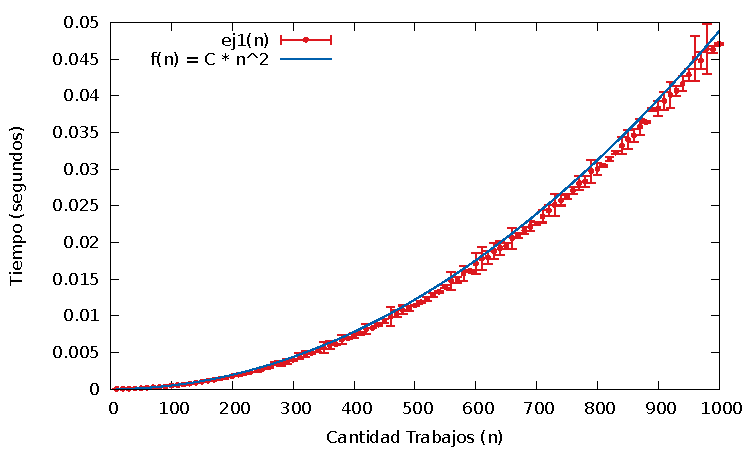
\includegraphics{imgs/ej1_1000_10_100.pdf}
\caption{Test Performance: Tiempo(s) vs Cantidad de Trabajos.}
\end{figure}

\par{Hay que notar que las franjas para cada tamaño de entrada muestran el desvío estandar de todos los valores conseguidos para ese tamaño, esto nos pareci\'o mucho m\'as significativo que simplemente mostrar el máximo y el m\'inimo, ya que estos valores pueden variar mucho por otros procesos que pueda estar ejecutando la computadora a la vez.}

\newpage

%\usepackage{amsmath} %<-- ajaja quien puso esto aca??
\section{Ejercicio 2}

\subsection{Interpretación del enunciado}
\par{Se tienen una cantidad $n$ de cursos con sus respectivas fechas de inicio y finalizaci\'on representadas con n\'umeros enteros positivos. El objetivo de este ejercicio es desarrollar un algoritmo que, dadas las fechas de inicio y fin de cada curso, encuentre un subconjunto de cursos que no se solapen entre s\'i, es decir, sean compatibles. Se pide que la complejidad del algoritmo sea estrictamente menor a O($n$^{2})$ siendo $n$ la cantidad de cursos$.}
\par{Para este ejercicio, asumiremos que los cursos no se interrumpen. Es decir, por ejemplo, que el curso que arranca el día 5 y termina el día 8 va a dictarse también los días 6 y 7. Entonces lo que nos queda es un problema de optimización: ¿Cómo elegir la mayor cantidad de cursos posibles de manera que ningún par de cursos dado tenga días en común?. En particular para que se puedan tomar dos cursos, la fecha de inicio de uno de los dos tiene que ser mayor (estricto) que la fecha de finalizacon del otro curso.}
\par{Cabe destacar que lo que este problema busca es maximizar la cantidad de cursos disponibles para ser cursados por un único alumno, y no buscar que haya más días cubiertos por un curso. También hay que mencionar que los cursos no tienen ningún valor numérico asignado.}
%	PONER EJEMPLOS

\subsection{Resolución}
\par{Para resolver este ejercicio se desarroll\'o un algoritmo goloso. Se busca devolver un conjunto de cursos. El algoritmo itera agregando, en caso de ser posible, un curso en cada iteraci\'on. Mientras se pueda seguir agregando cursos (no se puede si todos los restantes se solapan con alguno seleccionado), se agrega de los que quedan, el de menor fecha de finalizaci\'on que no se solape con alguno seleccionado. Luego se devuelven los cursos seleccionados.}
\par{A continuación expondremos un pseudocódigo de la solución implementada. Suponemos los datos levantados directamente desde la entrada y almacenados en un vector de cursos llamado $cronograma$.}\

%~ \begin{algorithm}[H]
%~ \SetLine
%~ \hspace{-13pt}\textbf{cronograma} resolver(\textbf{cronograma} $C$)\\
%~ C $\longleftarrow$ ordenar$\_$finalización($C$)\\
%~ $ultimaFecha \longleftarrow -1$\\
%~ $cronograma\_aceptado \longleftarrow \emptyset$\\
%~ \ForEach{c $\in$ C}{
  %~ \If{$fechaInicio(c) > ultimaFecha$}{
        %~ $cronograma\_aceptado \longleftarrow cronograma\_aceptado \cup c$\\
        %~ $ultimaFecha \longleftarrow fechaFin(c)$\\
  %~ }
%~ }
%~ \textbf{return} $cronograma\_aceptado$\\
%~ \caption{Resolución Golosa Ejercicio 2}
%~ \end{algorithm}
%~ 
\begin{algorithm}[H]
	\caption{Resolución Golosa Ejercicio 2}
	\begin{algorithmic}
		\KwData{vector(Curso) $entrada$}\\
		vector(Curso) $cronograma\_aceptado \longleftarrow \emptyset$\\
		\While{$puedoAgregarCursos$}{ 
			$cronograma\_aceptado \longleftarrow cronograma\_aceptado$ \cup\\
			$c \in entrada$ / $sonCompatibles(c, cronograma\_aceptado)$ \land \\
							$fechaFin(c) \geq fechaFin(c')$ \forall c'$ \in$ $entrada$
		}
		\textbf{return} $cronograma\_aceptado$\\
	\end{algorithmic}
\end{algorithm}
\par{El vector de cursos $entrada$ contiene todos los cursos de la instancia, mientras que el vector $cronograma\_aceptado$ contiene los que se van agregando a la soluci\'on. La funci\'on $sonCompatibles$ devuelve si el curso $c$ no se solapa con alg\'un curso del vector de aceptados.}

%~ \subsection{Complejidad}
%~ En lo que a complejidad se refiere, los fragmentos más costosos de nuestro algoritmo son la función ordenar$\_$finalización (l.2) y el ciclo que recorre linealmente todos los cursos $c$ dentro del cronograma $C$ (l.5). La función ordenar$\_$finalización está implementada mediante la función \textfff{sort} dentro de la STL de \textfff{C++}. La misma tiene una complejidad de $O(n log n)$ \footnote{http://www.cplusplus.com/reference/algorithm/sort/}. El ciclo de que recorre todos los cursos del cronograma $C$ tiene una complejidad de $O(n)$, ya que implementamos el cronograma sobre un vector. Luego, la complejidad de nuestra función resolver termina siendo de $T(n) = O(n log n) + O(n) = O(n log n)$.

\subsection{Complejidad}
\par{Para obtener en cada iteraci\'on del ciclo principal (l\'inea 2) el curso con menor fecha de finalizaci\'on, se pueden ordenar, antes de entrar al ciclo, los cursos seg\'un su fecha de finalizaci\'on. Ordenar los cursos puede hacerse en $O(n log n)$ con $n$ la cantidad de elementos a ordenar, en este caso, la cantidad de cursos de la entrada. Luego, con los cursos ordenados, el ciclo debe iterar sobre los $n$ cursos, evaluando si cada uno es compatible con el resto del cronograma aceptado. Esto puede hacerse determinando si se solapa con el anterior (como se agregan en orden, si se solapa con alguno, tiene que ser con el \'ultimo agregado), lo cual tiene complejidad O(1), ya que es una comparaci\'on de enteros (la fecha de finalizaci\'on del curso que se itera y la del \'ultimo curso agregado). Entonces, El ciclo que recorre los $n$ cursos del cronograma de entrada tiene una complejidad de $O(n)$. Luego, la complejidad de la función $resolver$ termina siendo de $T(n) = O(n log n) + O(n) = O(n log n)$.}

\subsection{Implementaci\'on}
\par{La implementaci\'on de este algoritmo en C++ primero ordena los cursos seg\'un su fecha de finalizaci\'on. Luego recorre todos los cursos en orden y para cada curso, eval\'ua si puede ser agregado o no. La función de ordenamiento está implementada mediante la función \textfff{sort} dentro de la STL de \textfff{C++}. La misma tiene una complejidad de $O(n log n)$ \footnote{http://www.cplusplus.com/reference/algorithm/sort/}. En cada iteraci\'on del ciclo que recorre los cursos, no hace m\'as que comparar la fecha de finalizaci\'on del curso que se itera con la del \'ultimo curso agregado. Si es mayor estricta, agrega el curso a los cursos aceptados.}

\subsection{Demostraci\'on de Correctitud}
\par{En esta secci\'on vamos a demostrar que el algoritmo resuelve el problema de encontrar la m\'axima cantidad de cursos que no se superponen.
Para eso demostraremos las siguientes propiedades:}

\begin{itemize}
\item \textbf{Prop 1: }\emph{Sea B un conjunto de cursos que maximiza la cantidad de cursos compatibles, y sea A el conjunto que siempre elige la de menor fecha de finalizaci\'on que sea compatible, \#A = \#B.}
\item \textbf{Prop 2: }\emph{Nuestro algoritmo siempre elige la de menor fecha de finalizaci\'on que sea compatible.}\\
\end{itemize}

%\textbf{1. Sea B un conjunto de cursos que maximiza la cantidad de cursos compatibles,
%   y sea A el conjunto que siempre elige la de menor fecha de finalizaci\'on que sea compatible. Luego \#A = \#B.}\\
%Para esto veremos que una solucion al problema reside en tomar el curso de menor fecha de finalizacion que sea compatible con
%los cursos tomados hasta el momento de la seleccion y encontrar la maxima cantidad de cursos que sean compatibles con el curso que acabamos de elegir.

\textbf{Prop 1)} Para demostrar esto, emplearemos la siguiente notaci\'on: Sea A = $\{A_1,A_2,A_3...A_k\}$ el conjunto de cursos que da nuestro algoritmo, donde se cumple que:
\begin{equation}
fechaFin(A_i)<fechaFin(A_j) \quad \forall i\textlessj ,1\le i<j\le k\\
\end{equation}
con $k$ la cantidad de cursos de nuestra soluci\'on; y definiendo a B = $\{B_1,B_2,B_3..B_m\}$, donde:\\
\begin{equation}
fechaFin(Ai)\textless fechaFin(A_j) \quad \forall i<j, 1\le i<j\le m\\ 
\end{equation}
con $m$ la cantidad de cursos de la soluci\'on \'optima, como B es el conjunto de cursos de la soluci\'on \'optima vale que $k\le m$ .\\

\textbf{Lema:} $FechaFin(A_i) \le FechaFin(B_i)$ $\forall i: 1\le i \le k$. Probaremos esto por inducción. Queremos ver que:
\begin{equation}
	fechaFin(A_i)\leq fechaFin(B_i) \quad \forall i: 1\le i \le k 
\end{equation}

Tomamos como caso base $fechaFin(A_1)\leq fechaFin(B_1)$. Esto es cierto ya que al inicio del algoritmo, cualquier curso es compatible (ya que el conjunto de cursos seleccionados hasta ese momento es vac\'io) y adem\'as el algoritmo siempre selecciona el curso compatible con menor fecha de finalizaci\'on. Luego queda probado el caso base.\\

Nuestro paso inductivo requiere probar que:
\begin{equation}
\forall c : 1 \le c < k \quad fechaFin(A_c)\leq fechaFin(B_c) \quad \Rightarrow fechaFin(A_{c+1})\leq fechaFin(B_{c+1})
\end{equation}

Como vale la hip\'otesis inductiva sabemos que $fechaFin(A_c)\leq fechaFin(B_c)$. Tambi\'en sabemos que la $fechaFin(B_{c+1}) > fechaInicio(B_{c+1})$ y, como B es un conjunto que tiene a cursos compatibles tenemos que $fechaInicio(B_{c+1}) > fechaFin(B_c)$. Luego con la afirmaci\'on anterior sumada a la hip\'otesis inductiva podr\'iamos seleccionar el curso $B_{c+1}$:

	  \begin{equation}
		fechaFin(A_c) \stackrel{\rm{por HI}} \le  fechaFin(B_c) \stackrel{\rm{B conj compatible}} < fechaInicio(B_{c+1})   \\ 
	\end{equation}
	  \\ Ya que nuestro algoritmo selecciona el curso compatible con menor fecha de finalización, se deduce
	  que $fechaFin(A_{c+1})\le fechaFin(B_{c+1})$ \Box \\
	  
	
Con el lema podremos probar que vale que $k\ge m$, y como sab\'iamos que $k\le m$ tendremos que el conjunto
de soluciones dadas por el algoritmo es \'optimo en cuanto a maximizar la cantidad de cursos que sean compatibles. Demostraremos, a continuación, que $K\ge m$, por el absurdo.\\ 

Sea $B$ el conjunto que maximiza la cantidad de cursos con un cardinal de $m$, y el conjunto que devuelve nuestro algoritmo un cardinal de $k$. Supongamos que $k<m$ y lleguemos a un absurdo.
Como $B$ es un conjunto que tiene cursos compatibles, el curso $B_{k+1}$ es compatible con el conjunto $\{B_1,B_2,B_3..B_k\}$. Del lema sabemos que $FechaFin(A_k) \le fechaFin(B_k)$, por lo tanto $B_{k+1}$ tambi\'en ser\'ia compatible con el conjunto $\{A_1,A_2,A_3..A_k\}$. Luego, ese curso entraria en el cronograma de cursos acepatados de nuestro algoritmo. Esto es un absurdo, ya que supusimos que $\#A = k$ \Box\\


\textbf{Prop 2)} Es preciso notar que nuestro algoritmo ordena en forma creciente de acuerdo a la fecha de finalizaci\'on y luego recorre desde el de menor fecha, hasta el de mayor fecha de finalizaci\'on. Por otro lado siempre elige tomar un curso m\'as, si este es compatible ya que de la forma que recorremos vale que:
\begin{equation}
fechaFin(curso_{iteracionj}) \geq fechaFin(curso_{iteracioni}) \quad \forall j>i
\end{equation}


Adem\'as el algoritmo en cada iteraci\'on comprueba que: 
\begin{equation}
fechaInicio(curso_{iteracionj}) > ultimaFechaFin 
\end{equation}
para que no haya solapamientos entre el curso a elegir con los ya elegidos anteriormente.\\
Esto es v\'alido debido a que la $fechaInicio(curso_{iteracionj}) > ultimaFechaFin $ y\\
$fechaFin(curso_{iteracionj}) \geq fechaFin(curso_{iteracioni}) \quad \forall j>i$\\

\newpage
\subsection{Testing}
\textbf{Correctitud}\\
Los tests expuestos a continuación fueron diseñados con el fin de verificar diferentes casos particulares que pudimos identificar. Para cada test vamos a exponer la entrada, la salida y, en caso de que sea necesario, una justificaci\'on de la correctitud de la soluci\'on.\\

\noindent\textbf{Test$\#$1}\\
\textbf{Caracterización:} Varios cursos que no coinciden en ningún dia.\\
\textbf{Input:} \textfff{4 1 2 3 4 5 6 7 8}\\
\textbf{Output:} \textfff{1 2 3 4}\\
\textbf{Status:} OK. Los 4 cursos se pueden tomar.\\

\noindent\textbf{Test$\#$2}\\
\textbf{Caracterización:} Varios cursos, todos incompatibles entre si.\\
\textbf{Input:} \textfff{3 1 5 2 6 3 7}\\
\textbf{Output:} \textfff{1}\\
\textbf{Status:} OK. Si bien elegir cualquiera de los cursos es solución, nuestro algorimo elije el primero analizado.\\

\noindent\textbf{Test$\#$3}\\
\textbf{Caracterización:} Prioriza obtener la mayor cantidad de cursos, por sobre la mayor cantidad de horas cursadas.\\
\textbf{Input:} \textfff{4 9 15 3 7 21 27 1 31}\\
\textbf{Output:} \textfff{2 1 3}\\
\textbf{Status:} OK. Se descarta el curso que dura desde el 1ro hasta el 31 del mes, para que se puedan dictar los 3 cursos que no se solapan entre si.\\

\noindent\textbf{Test$\#$4}\\
\textbf{Caracterización:} Cursos encadenados.\\
\textbf{Input:} \textfff{11 1 2 2 3 3 4 4 5 5 6 6 7 7 8 8 9 9 10 10 11 11 12}\\
\textbf{Output:} \textfff{1 3 5 7 9 11}\\
\textbf{Status:} OK. Se preserva la mayor cantidad de cursos, eliminando los necesarios para ``desconectar'' toda la serie. En estos casos, hay que eliminar un curso de por medio.\\

\newpage
\textbf{Performance}\\
\par{Para realizar los tests de performance escribimos un programa (\textfff{testGen.cpp}) que genera de manera aleatoria varias instancias de prueba para cada $n$ entre 1 y 1000000 con un salto de 10000(20 mediciones por cada n). Para poder visualizar de la mejor manera posible la curva de performance de nuestro programa, programamos nuestro generador para que produzca tests en el peor caso posible\footnote{Las mediciones de tiempos de las instancias se encuentran en codigo/ej2/tests/test.out}. Para ese ejercicio, y viendo que la complejidad de nuestro algoritmo viene dada por la operación de ordenamiento, decidimos generar los tests de modo tal que las fechas de inicializacion y finalizacion de cada curso sea aleatoria. En el gráfico agregamos la función $f = C * n log (n)$ donde C = $\frac{1}{37500000}$ } que acota por arriba a la media de las mediciones.

\begin{figure}[H]
\centering
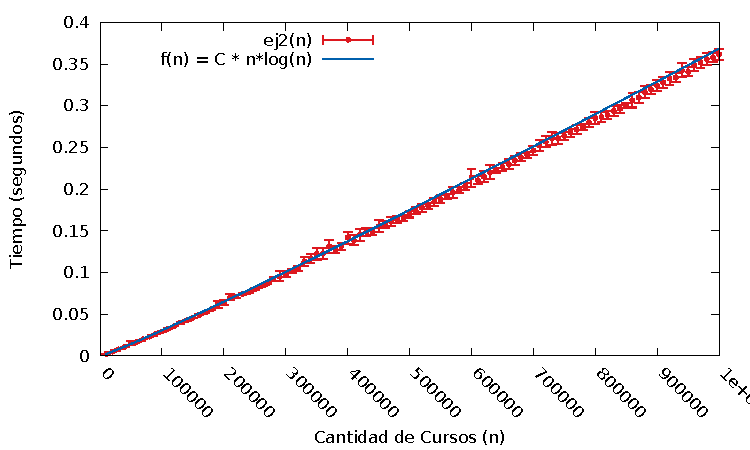
\includegraphics{imgs/ej2.pdf}
\caption{Test de Performance: Tiempo(s) vs Cantidad de Cursos}
\end{figure}


\newpage

\section{Ejercicio 3}
\subsection{Interpretación del enunciado}
\par{En cierta provincia se ubican varias fábricas de ladrillos pertenecientes
  una misma empresa. La empresa se encarga de distribuír  lo s ld rillos de l
as fábricas a sus clientes. Para ello, utiliza las rtas provinciales que conec                                                                                                                                                                                                                                                                                         
distintos puntos de la provincia en los que puede haber una fábrica o un
cliente. Sin embargo, las rutas no están preparadas para soportar el peso de
los camiones que transportan los ladrillos, así que estas deben ser
fortalecidas. El costo de fortalecer cada ruta es proporcional a la longitud de
la misma. La empresa quiere fortalecer determinadas rutas para poder distribuír
los ladrillos a sus clientes sin problemas, intentando reducir lo más posible
el costo de dicha remodelación. El objetivo del ejercicio es desarrollar un
algoritmo que determine el conjunto de rutas que deben ser fortalecidas para
poder continuar la distribución (debe haber una ruta fortalecida entre cada
cliente y al menos una fábrica), cuyo costo de fortalecimiento sea mínimo.}
\subsection{Resolución}
\par{Se modelará la situación a través de un grafo en el que cada nodo
representará un cliente o una fábrica y cada arista entre un par $v1$, $v2$
de nodos representará una ruta entre los clientes o fábricas correspondientes a
$v1$ y $v2$. Para modelar el costo de fortalecer cada ruta, se le asignará a
cada arista el peso equivalente a la longitud de su correspondiente ruta. Si
bien el grafo podría no ser conexo, Se asume que existe un camino simple entre
cada cliente y al menos una fábrica, ya que se parte de que se puede satisfacer
la demanda de todos los clientes. Se busca obtener un conjunto de rutas tal que
exista un camino entre cada cliente y al menos una fábrica, es decir que
debemos encontrar un subgrafo en el grafo modelado. Como se busca reducir el
costo total sería conveniente que dicho subgrafo esté compuesto por árboles.
Este subgrafo constaría de una componente conexa por cada fábrica, sin dejar
clientes afuera. Cada componente conexa tendría que ser un árbol generador
del subgrafo inducido por los nodos de dicha componente. De esta forma se está
asegurando mantener la mínima cantidad de rutas necesarias. De todos los
posibles subgrafos bosque, debemos tomar el de menor peso para reducir el costo
total de fortalecer las rutas. En definitiva hay que encontrar un bosque
generador (conjunto de árboles generadores) de peso mínimo en el grafo modelado,
con la restricción de que haya exactamente una fábrica en cada árbol y ningún
cliente quede afuera.

A continuación, se presenta el pseudocódigo del algoritmo:\\

\begin{algorithm}[H]
	\caption{Algoritmo de Ejercicio 3}
	\KwData{Grafo G=(V,E) con nodos clientes y nodos fábrica, tal que para todo cliente, hay una fábrica alcanzable desde el.}
	
	$G.aristas \longleftarrow$ ordenar$\_$por$\_$peso$\_$asc($G.aristas$)\\
	\textbf{vector<arista>} $res \longleftarrow \emptyset$\\
	\ForEach{$e \in G.aristas$}{
		\If{!forma$\_$ciclo($e$, $res$) $\land$ no une dos componentes con una fábrica en cada una}{
		$res \longleftarrow res \cup e$\\
		}
	}
	\textbf{return} $res$\\
	
\end{algorithm}

}

\subsection{Demostración de Correctitud}


\textbf{La solución es válida:\\}
    Demostración:
    Todo cliente puede ser provisto por al menos una fábrica ya que hay una
    fábrica por componente conexa.
    Veremos que el algoritmo retorna un grafo $G $con cada cliente que pertenece a una componente
    conexa(en la que hay una fábrica):\\
    Supongamos que hay un cliente $c$ que no está en ninguna componente conexa. Esto es equivalente a afirmar
    que $c \notin V(G)$. Como cada cliente en el grafo de entrada del algoritmo, tiene un camino a alguna fábrica
    $\Longrightarrow$ existe un camino entre cualquier cliente y alguna fábrica.}

\textbf{Demostrar que es óptimo}

    \par{
%   \textbf{Demostrar que existe una solución óptima con una fábrica por componente conexa:}
    
    Notar que la solución debe cumplir que en cada componente conexa hay al menos una fábrica. Veremos que si un grafo $G$ contiene
    más de una fábrica en una componente conexa, existe un subgrafo (con el mismo conjunto de vertices y menos aristas)
    de $G'$ con una sola fábrica por componente conexa con menor peso que el de $G$.
    
    \textbf{Propiedad:} Sea una $G$ el grafo de una solución con más
    de una fábrica en alguna componente conexa, veremos que si hay una sola fábrica en esa componente, el costo de la nueva solución
    quitandole una arista \footnote{Esta arista que quitamos pertence a un camino entre dos fábricas}tiene igual o menor peso.\\
    
    Demostración:
    Sea $P$ un camino entre dos fábricas y sea $G'$ el grafo resultante de quitarle una arista $e$ (que une a los nodos $u,v$)
    perteneciente a un camino entre dos fábricas:$ P = C_1 \leftrightarrow (u,v) \leftrightarrow C_2$.
    Veamos que $G'$ sigue siendo solución posible.
    
    Sea un nodo cliente que no está en la componente conexa a la que pertenece $e$. Luego, ese cliente tiene a una fábrica alcanzable,
    ya que no quitamos ninguna arista de su componente conexa y como $G$ era solución, había una fábrica en esa componente.
    Sea un nodo cliente $c$ que estaba en la componente conexa a la que pertenece $e$.
    En ese caso como $G$ era un grafo solución, existia en $G$ un camino entre un c y una fábrica. Luego en ese camino, pasaba por
    $u$, o por $v$ (los nodos incidentes a la arista removida).Sin perdida de generalidad, supongamos que inicidía en v.
    
    Como $e$ era una arista que pertenecía a un camino entre dos fábricas se puede crear un camino
    que llegue desde $c$ a una fábrica: $ c \leftrightarrow v \leftrightarrow C_2$. Luego $G'$ tambien es solución.
    Además como quitamos una arista, que tiene peso positivo (todas lo tienen), el costo
    de la solución es menor o igual a la solución anterior.
    
    Esta quita de aristas se puede repetir hasta tener un grafo con una fábrica por componente conexa. Este grafo
    sera solución optima pues no se le pueden quitar aristas: si se remueve una arista de una componente conexa (que es un arbol) 
    la cual contiene una sola fábrica , se va a desconectar la componente generando asi la imposibilidad
    para algun cliente de alcanzar a la fábrica que estaba en la componente conexa (antes de quitar la arista).\\}

% 	\par{\textbf{Demostrar que usa la cantidad mínima de aristas:}
% 	Sea T una solución con una fábrica por componente conexa(cc) y c aristas (la cantidad de cliente).
% 	Como cada cc es una AGM, al quitar una arista de una cc, pasan a haber 2 ccs, y como sólo había una fábrica por cc,
% 	los clientes de alguna de las 2 ccs formadas no podrá ser provisto.
% 	$\Rightarrow$ La cantidad de aristas de la solución es mínima.}

  \par{
  \textbf{El peso de la solución es mínimo:\\} 
  Demostración:\\
  Sea $T$ la solución devuelta por nuestro algoritmo y sea $e$ una arista del grafo original tal que $e \notin T$.
  Agrego la arista $e = (u,v)$ a $T$ generando así al grafo $T'$:

  \textbf{Caso 1, $u$ y $v$ pertenecen a la misma cc en T: } 
  Cada cc del grafo devuelto por nuestro algoritmoes un AGM y, por ser árbol,
  $T+e$ contiene un ciclo incluído en la cc de $u$ y $v$. Sea $C$ tal ciclo, tomo $f$
  arista en $C$. Defino $T' = T+e-f$ con peso $p(T') = p(T) + p(e) - p(f)$.
  Como nuestro algoritmo siempre selecciona las aristas de peso minimo que no forman ciclo
  $$p(f) \leq p(e)$$ , luego
  $$0 \leq p(e) - p(f) \Rightarrow p(T') \geq P(T)$$. Es preciso aclarar que $T+e-f$ es conexo, por lo tanto todos los clientes
  tienen a una fábrica alcanzable.

  \textbf{Caso 2, $u$ y $v$ pertenecen a distintas cc en T: }
  Las ccs de $u$ y $v$ ahora son una misma cc con dos fábricas. Esta cc es un árbol porque es conexa (obvio) y la cantidad de
  aristas es la suma de la cantidad de aristas es $m = m1+m2+1 = n1-1 + n2-1 +1 = n1+n2-1 = n-1$.
  Luego puedo quitar una arista que pertenece al camino entre las dos fábricas \footnote{Es preciso aclarar que puedo suponer esto de la arista
  que quitamos ya que nuestro algoritmo no devuelve grafos con componentes conexas con más de una fábrica.}
  que actualmente están conectadas con el  camino
  $ P = C_1 \leftrightarrow (u,v) \leftrightarrow C_2$. Luego cualquier cliente del grafo resultante de remover la arista $e$
  tiene un camino hasta alguna fábrica:
  
  Sea un nodo cliente que no está en la componente conexa a la que pertenece $e$. Luego, ese cliente tiene a una fábrica alcanzable,
  ya que no quitamos ninguna arista de su componente conexa y como $T$ era solución, había una fábrica en esa componente.
  
  Sea un nodo cliente $c$ que estaba en la componente conexa a la que pertenece $e$.
  En ese caso como $T$ era un grafo solución, existia en $T$ un camino entre un c y una fábrica. Luego en ese camino, pasaba por
  $u$, o por $v$ (los nodos incidentes a la arista removida).Sin perdida de generalidad, supongamos que inicidía en v.
    
  Como $e$ era una arista que pertenecía a un camino entre dos fábricas se puede crear un camino
  que llegue desde $c$ a una fábrica: $ c \leftrightarrow v \leftrightarrow C_2$. Luego $T'$ tambien es solución.
    
  Como nuestro algoritmo siempre selecciona las aristas de peso minimo que no forman ciclo
  $$p(f) \leq p(e)$$ , luego
  $$0 \leq p(e) - p(f) \Rightarrow p(T') \geq P(T)$$.
    
% 		Como la cantidad de aristas
% 		de la solución actual es una más que la mínima puedo sacar una arista de la nueva cc para obtener una solución mejor que
% 		T+e, siempre y cuando mantenga que las dos ccs que se formen al quitar una arista de la nueva cc, tengan una fábrica.
% 		Sea f una arista distinta de e tal que al quitarla de la nueva cc, se formen dos ccs con una fábrica cada una (Si no hubiese
% 		una f distinta de e, tendría que sacar e y volvería a quedar la misma solución, por lo tanto sería solución única).
% 		el peso de f no puede ser mayor al peso de e porque si lo fuera, en lugar de escoger f, el algoritmo habría escogido e.\\
}


    $\Rightarrow$ Cualquier solución del tipo $T+e-f$ tiene peso mayor o igual al peso de $T \Rightarrow$ Nuestra solución es óptima. \box

}

\end{enumerate}

%\subsection{Complejidad}
%La complejidad del algoritmo es $O(m+n)$, ya que se fija en todas las aristas

\subsection{Cota de Complejidad}

\subsection{Implementación}

\begin{lstlisting}
grafo kruskal(){
  disjointSet ds(this->cantNodos);
  vector<arista> res;
  /*Ordeno la lista de aristas para Kruskal */ // ----> O(n logn)
  sort(this->aristas.begin(), this->aristas.end()); 
  
  int i = 0;	//indice de arista que itero
  int j = 0;	//Cantidad de aristas que agregue
  int cantClientes = cantNodos - this->cantFabricas;
  
  while (j < cantClientes){
    int root1 = ds.root(this->aristas[i].nodo1)->valor;
    int root2 = ds.root(this->aristas[i].nodo2)-> valor;
    if((root1 != root2) 	//estan en distintas componente conexas y...
    // no pasa que ambos tengan una fabrica
    && !((root1 < this->cantFabricas) && (root2 < this->cantFabricas)) ){ 
      if (root1 < this->cantFabricas) {  //Si el primero es una fabrica...
	      ds.simple_join(root2, root1);      
      } else {   //Si el segundo es fabrica o si ninguno lo es.
	      ds.simple_join(root1, root2);	     
      }
      j++;
      res.push_back(this->aristas[i]);
    }
    i++;
  }
  
  /* Armo el grafo para devolver */
  grafo g_res(this->cantNodos);
  for(int i = 0; i < res.size(); ++i)
	  g_res.asociar(res[i].nodo1+1, res[i].nodo2+1, res[i].peso);
  
  return g_res;
}
\end{lstlisting}
\newpage


\subsection{Testing de Correctitud}

Los tests expuestos a continuación fueron diseñados con el fin de verificar
diferentes casos particulares que pudimos identificar. Para cada test vamos
a exponer la entrada, la salida y, en caso de que sea necesario, una
justificaci\'on de la correctitud de la soluci\'on.\\

\noindent\textbf{Test$\#$1}\\
\textbf{Caracterización:} Una fábrica sin clientes.\\
\textbf{Input:}\\ \texttt{1 0 0}
\begin{center}
\begin{dot2tex}
graph graphname{
	rank=same;
	rankdir="LR";
	splines=line;
	1;
}
\end{dot2tex}
\end{center}
\textbf{Output:} \texttt{0 0}\\
\textbf{Status:} Ok, como no hay clientes, no hay rutas que fortalecer.\\

\noindent\textbf{Test$\#$2}\\
\textbf{Caracterización:} Varias fábricas sin clientes.\\
\textbf{Input:}\\ \texttt{6 0 8\\1 2 5\\1 3 7\\2 3 3\\2 4 6\\3 4 8\\
4 5 8\\4 6 4\\6 1 2}
\begin{center}
\begin{dot2tex}
graph graphname{
	rank=same;
	rankdir="LR";
	splines=line;
	1 -- 2 [label=5];
	1 -- 3 [label=7];
	3 -- 2 [label=3];
	4 -- 2 [label=6];
	4 -- 3 [label=8];
	5 -- 4 [label=8];
	4 -- 6 [label=4];
	1 -- 6 [label=2];
}
\end{dot2tex}
\end{center}
\textbf{Output:} \texttt{0 0}\\
\textbf{Status:} Ok, como no hay clientes, no hay rutas que fortalecer.\\



\noindent\textbf{Test$\#$3}\\
\textbf{Caracterización:} Varias fábricas y un cliente.\\
\textbf{Input:}\\ \texttt{4 1 8\\1 2 5\\1 3 7\\2 3 3\\2 4 6\\3 4 8\\
4 5 8\\4 1 4\\5 2 2}
\begin{center}
\begin{dot2tex}
graph graphname{
	rank=same;
	rankdir="LR";
	splines=line;
	1 -- 2 [label=5];
	1 -- 3 [label=7];
	3 -- 2 [label=3];
	4 -- 2 [label=6];
	4 -- 3 [label=8];
	5 -- 4 [label=8];
	4 -- 1 [label=4];
	2 -- 5 [label=2];
}
\end{dot2tex}
\end{center}
\textbf{Output:} \texttt{ 2 1 5 2}\\
\textbf{Status:} Ok, como hay un solo cliente (el nodo 5), elige la ruta de costo minimo que conecta
 a ese cliente con una de las fábricas(el nodo 2) adyacentes.\\

\noindent\textbf{Test$\#$4}\\
\textbf{Caracterización:} Varios clientes y una fábrica.\\
\textbf{Input:}\\ \texttt{1 4 8\\1 2 5\\1 3 7\\2 3 3\\2 4 6\\3 4 8\\
4 5 8\\4 1 4\\5 2 2}
\begin{center}
\begin{dot2tex}
graph graphname{
	rank=same;
	rankdir="LR";
	splines=line;
	1 -- 2 [label=5];
	1 -- 3 [label=7];
	3 -- 2 [label=3];
	4 -- 2 [label=6];
	4 -- 3 [label=8];
	5 -- 4 [label=8];
	4 -- 1 [label=4];
	2 -- 5 [label=2];
}
\end{dot2tex}
\end{center}
\textbf{Output:} \texttt{14 4 5 2 2 3 4 1 1 2 }\\
\textbf{Status:} Ok, como hay una sola fábrica debe conectar a todo el grafo(fábrica y clientes) con el menor costo posible.
Es decir debe hacer el AGM del grafo. Notar que lo hace ya que devuelve lo que haria Kruskal, siempre eligiendo los nodos de menor peso
que no generan circuitos.\\

\newpage
\subsection{Testing de Performance}

Para realizar el test, generamos grafos aleatorios, con pesos aleatorios (entre 0 y 100). Decimos que los grafos son aleatorios, porque nuestro algoritmo va agrandando alguna componente conexa uniendo vertices
correspondientes a los clientes con componenetes conexas que contienen una fabrica. Cabe destacar que esas componenetes conexas pueden ser simplemente una fábrica.

Realizamos un gráfico comparando la sucesión de tiempos obtenida con una función cuadrática.
La función $f = C * n^2$, donde C es una constante. Se midió el tiempo con n desde 1 hasta 1000 con saltos de a 10 (con 10 mediciones por cada n).\\

\begin{figure}[H]
\centering

\includegraphics{imgs/logo_dc.jpg}
\caption{Test Performance: Tiempo(s) vs Cantidad de Clientes y Fábricas.}
\end{figure}

\newpage

\section{Conclusiones}

La realización de este trabajo práctico nos permitió familiarizarnos con el enfoque teórico-experimental que la cátedra espera dentro de los trabajos prácticos. Pudimos recorrer el proceso del análisis formal de un problema, desde su observación inicial hasta las conclusiones prácticas. 

Por el lado teórico y formal, nos planteó las dudas sobre que es necesario demostrar para justificar nuestras soluciones propuestas. Por el lado práctico, nos ayudó a complementar las nociones de algoritmos greedy y backtracking que ya habíamos visto en las clases teóricas de la materia.

También nos acercó ciertas nociones preliminares sobre cómo mostrar resultados de la manera más concreta posible y evitar los errores más comunes al hacerlo.

Para finalizar, sentimos que este trabajo nos representó un buen ejercicio en el análisis algorítmico general y nos dejó bien orientados para afrontar los siguientes proyectos dentro de la materia.

\end{document}
